
%\documentclass[a4paper,nobib,justified]{tufte-book}
\documentclass[a4paper,nobib,justified,notoc]{tufte-book}
\usepackage[natbib=true,backend=biber,style=authoryear-icomp,citestyle=authoryear-icomp]{biblatex}

\title{PhD Thesis}
\author{YOUR NAME}

\hypersetup{colorlinks}


\usepackage[utf8]{inputenc}
\usepackage[T1]{fontenc}
\usepackage{graphicx}
\usepackage{textcomp}
\usepackage{booktabs}
\usepackage[nottoc,notlof,notlot]{tocbibind}
\usepackage{minitoc}

\usepackage{lipsum}

\setcounter{secnumdepth}{3}
\setcounter{tocdepth}{3}

\addbibresource{pubs_biblio.bib}

% \graphicspath{{./figures-bin/}{./figures/}{./images/}{./figures/chapters/}}
\graphicspath{{./figures/}{./images/}{./figures/chapters/}}

%%%%%%%%%%%%%%%%%%%%%%%%%%%%
%New commands
\newcommand{\blankpage}{\newpage\hbox{}\thispagestyle{empty}\newpage}

%%%%%%%%%%%%%%%%%%%%%%%%%%%
%Redefinition of environments
\makeatletter
    \if@compatibility
\renewenvironment{titlepage}
    {%
      \cleardoublepage
      \if@twocolumn
        \@restonecoltrue\onecolumn
      \else
        \@restonecolfalse\newpage
      \fi
      \thispagestyle{empty}%
      %\setcounter{page}\z@
    }%
    {\if@restonecol\twocolumn \else \newpage \fi
    }
\else
\renewenvironment{titlepage}
    {%
      \cleardoublepage
      \if@twocolumn
        \@restonecoltrue\onecolumn
      \else
        \@restonecolfalse\newpage
      \fi
      \thispagestyle{empty}%
      %\setcounter{page}\@ne
    }%
    {\if@restonecol\twocolumn \else \newpage \fi
     \if@twoside\else
       % \setcounter{page}\@ne
     \fi
    }
\fi
\makeatother

\makeatletter
  \newenvironment{frontsection}[1][Abstract]{
  	\titlepage
    % \null\vfil
    %@beginparpenalty\@lowpenalty
    \begin{center}%
    \LARGE\textbf{#1}
    %@endparpenalty\@M
    \end{center}
    }%
    {\par\vfil\null\endtitlepage}
    %{\par\vfil\null}
\makeatother


\makeatletter% since we're using commands with @ in their name
\let\origappendix\appendix% save a copy of the original meaning of \appendix
\renewcommand{\appendix}{%
  \origappendix% do all the original \appendix stuff
  \titlecontents{chapter}%
    [0em] % distance from left margin
    {\vspace{1.5\baselineskip}\begin{fullwidth}\LARGE\rmfamily\itshape} % above (global formatting of entry)
    {\hspace*{0em}\appendixname~\thecontentslabel: } % before w/label (label = ``2'')
    {\hspace*{0em}} % before w/o label
    {\rmfamily\upshape\qquad\thecontentspage} % filler + page (leaders and page num)
    [\end{fullwidth}] % after
  \titleformat{\chapter}%
    [display]% shape
    {\relax\ifthenelse{\NOT\boolean{@tufte@symmetric}}{\begin{fullwidth}}{}}% format applied to label+text
    {\itshape\huge Appendix~\thechapter}% label
    {0pt}% horizontal separation between label and title body
    {\huge\rmfamily\itshape}% before the title body
    [\ifthenelse{\NOT\boolean{@tufte@symmetric}}{\end{fullwidth}}{}]% after the title body
  \setcounter{tocdepth}{1}
  \setcounter{secnumdepth}{1}
  %
  % Add any other special appendix-related code here.
  %
}
\makeatother% restore the special meaning of @

\DeclareCiteCommand{\citeauthor}
  {\boolfalse{citetracker}%
   \boolfalse{pagetracker}%
   \usebibmacro{prenote}}
  {\ifciteindex
     {\indexnames{labelname}}
     {}%
   \printtext[bibhyperref]{\printnames{labelname}}}
  {\multicitedelim}
  {\usebibmacro{postnote}}


\usepackage{changepage}
\strictpagecheck
\strictpagechecktrue


\makeatletter
\newcommand{\newcleardoublepage}{\clearpage\if@twoside
  \ifodd\c@page \hbox{}\newpage\if@twocolumn\hbox{}%
  \newpage\fi\fi\fi}
\makeatother

\usepackage{transparent}


\newcommand{\beforechapterpic}[3][]{%
  % \clearpage
  \newcleardoublepage

  % \checkoddpage
  % \ifoddpage
  % % \else
  %   % \mbox{}
  %   \clearpage
  % \fi
\begin{figure*}[p]
 {\includegraphics[width=\textwidth]{#2}}
  {\centering #3}
\end{figure*}
}
\newcommand{\beforechapterpicd}[3][]{%
  % \clearpage
  \newcleardoublepage

  % \checkoddpage
  % \ifoddpage
  % % \else
  %   % \mbox{}
  %   \clearpage
  % \fi
\begin{figure*}[p]
  % \includegraphics[width=\textwidth,draft]{{Missing watercolor illustrations will be finished and included later}}
  {\centering \bf Missing watercolor illustrations will be finished and included later}

  \vspace{2cm}

  {\centering #3}
\end{figure*}
}

\makeatletter
\newcommand*{\cleartoleftpage}{%
  \clearpage
    \if@twoside
    \ifodd\c@page
      \hbox{}\newpage
      \if@twocolumn
        \hbox{}\newpage
      \fi
    \fi
  \fi
}
\makeatother

\makeatletter
\newcommand*{\illustratedblankpage}{
~
% \vspace{2cm}
\vfill
\begin{figure*}
\begin{center}
% \includegraphics[width=\textwidth,draft]{images/defense.png}
% {\centering Thesis defense, Talence. December 2018}

\includegraphics[width=0.5\textwidth]{figures/agent.pdf}
\end{center}
\end{figure*}
\vfill}
\makeatother

\newcommand{\lastpic}[3][]{%
  % \clearpage
  % \clearpage
  % \checkoddpage
  % \ifoddpage
  % % \else
  %   % \mbox{}
  %   \clearpage
  % \fi
  \cleartoleftpage
\begin{figure*}[p]
  \includegraphics[width=\textwidth]{#2}
  {\centering #3}
\end{figure*}
}
\newcommand{\beforechapterdoublepic}[5][]{%
  % \clearpage
  \newcleardoublepage

  % \checkoddpage
  % \ifoddpage
  % % \else
  %   % \mbox{}
  %   \clearpage
  % \fi
\begin{figure*}[p]
  \includegraphics[width=\textwidth]{#2}
  {\centering #3}

\vspace{1cm}

  \includegraphics[width=\textwidth]{#4}
  {\centering #5}
\end{figure*}
}


\makeatletter
\renewcommand\@endpart{\vfil
              \if@twoside
                \null
                \thispagestyle{empty}%
                \newpage
              \fi
              \if@tempswa
                \twocolumn
              \fi}
\makeatother


\makeatletter
\newcommand{\partnoblank}[2][]{
\@openrightfalse
\part{#2}
\@openrighttrue}
\makeatother

\usepackage{eufrak}

% \newcommand{\chapterpic}[2][]{%
%   \checkoddpage
%   \ifoddpage
%     \newpage
%   \fi
%   \includegraphics[width=1.2\textwidth]{#3}
% }

\citetrackerfalse

\usepackage{color}
\usepackage{soul}
\setstcolor{red}

%pour corriger dans le texte, barre l'ancien texte et remplace par du texte en rouge
\newcommand{\corr}[2]{\st{#1}{{\textcolor{red}{#2}}}}

% met les notes en petit
\usepackage[textsize=scriptsize]{todonotes}

%commande pour PY pour qu'il puisse faire des commentaire
\newcommand{\todoPY}[1]{\todo[backgroundcolor=red!40, linecolor=red!40]{#1}}
\newcommand{\todoPYNL}[1]{\todo[backgroundcolor=red!40, noline]{#1}}
\newcommand{\todoPYIL}[1]{\todo[backgroundcolor=red!40, inline]{#1}}


\newcommand{\todoSB}[1]{\todo[backgroundcolor=red!40, linecolor=red!40]{#1}}
\newcommand{\todoSBNL}[1]{\todo[backgroundcolor=red!40, noline]{#1}}
\newcommand{\todoSBIL}[1]{\todo[backgroundcolor=red!40, inline]{#1}}

\newcommand{\todoNL}[1]{\todo[noline]{#1}}
\newcommand{\todoIL}[1]{\todo[inline]{#1}}

\usepackage{printlen}


\setcaptionfont{%
  \normalfont\footnotesize
}

\newcommand{\acrotable}[0]{\sidenote{A table of symbols, acronyms and abbreviations can be found at the last page of this manuscript.}}

\usepackage{algorithm}
\usepackage[noend]{algpseudocode}
% \algrenewcommand\textproc{}
\algnewcommand{\LeftComment}[1]{\Statex \(\triangleright\) #1}

\usepackage{stmaryrd}
\usepackage{array}
\usepackage{booktabs}
% \usepackage{makecell}
\usepackage{multirow}
\usepackage{multicol}
\usepackage{tabularx}
\newcolumntype{L}[1]{>{\raggedright\let\newline\\\arraybackslash\hspace{0pt}}m{#1}}
\newcolumntype{C}[1]{>{\raggedright\let\newline\\\arraybackslash\hspace{0pt}\centering}m{#1}}

\usepackage{enumitem}
\setlist{itemsep=0pt,font=\normalfont\textbf}

\pdfobjcompresslevel 0

\usepackage{csquotes}

\def\signed #1{{\leavevmode\unskip\nobreak\hfil\penalty50\hskip2em
  \hbox{}\nobreak\hfil(#1)%
  \parfillskip=0pt \finalhyphendemerits=0 \endgraf}}
\newsavebox\mybox
\newenvironment{aquote}[1]
  {\savebox\mybox{#1}\begin{quote}}
  {\vspace{0.1cm}\signed{\usebox\mybox}\end{quote}}

\usepackage{amsmath}
\DeclareMathOperator*{\argmax}{arg\,max}
\DeclareMathOperator*{\argmin}{arg\,min}

\hypersetup{%
  colorlinks = true,
  linkcolor  = DarkGreen
}



\usepackage{makeidx}
\makeindex

%\includeonly{}
\begin{document}
\sloppy
\dominitoc
\hypersetup{pageanchor=false}

{\let\cleardoublepage\clearpage
\pagestyle{empty}
\newgeometry{marginratio=1:1,vmarginratio=1:1}
\begin{titlepage}
     \vspace*{-96pt}
     \noindent \hspace{-48pt}
     
\includegraphics[height=72pt]{logo_ub.jpg}
     \hspace{148pt} 
\includegraphics[height=72pt]{logo_inria.jpg}
     \begin{center}
         \vspace{0.8cm}
         \large  TH\`{E}SE PR\'{E}SENT\'{E}E\\ POUR OBTENIR LE GRADE DE\\
         \vspace{0.5cm}
         \Large  {\bf DOCTEUR DE\\ L'UNIVERSIT\'{E} DE BORDEAUX}\\
         \vspace{1cm}
         \large \'{E}COLE DOCTORALE DE\\ MATH\'{E}MATIQUES ET INFORMATIQUE\\
         \vspace{0.5cm}
         \large SP\'{E}CIALIT\'{E} : INFORMATIQUE\\
         \vspace{1.2cm}
         \Large Par YOUR NAME\\
         \vspace{0.7cm}
         \rule{4em}{1pt}\\
         \vspace{0.7cm}
         \Large {\bf Your Thesis Title}\\
         \vspace{0.5cm}
         \rule{4em}{1pt}\\
         \vspace{0.7cm}
         \Large Sous la direction de : Your Advisor
         \vspace{0.5cm}
     \end{center}
     \vfill
     \noindent {\bf Date de soutenance : xx mois 20xx} \\
     ~\\
     \noindent {\bf Membres du jury :} \\
     ~\\
     \begin{tabular}{lll@{}}
         \textbf{Membre1} Président du jury/Rapporteur\\
         \textbf{Membre2} Rapporteur\\
         \textbf{Membre3} Examinateur\\
         \textbf{Membre4} Examinateur\\
         \textbf{Membre5} Invité\\
         \textbf{Membre6} Directeur de thèse\\
     \end{tabular}
\end{titlepage}
\restoregeometry
\cleardoublepage

\illustratedblankpage
}

\frontmatter\pagenumbering{roman}\pagestyle{empty}

\pagestyle{empty}
\newgeometry{marginratio=1:1,vmarginratio=1:1}

\hypersetup{pageanchor=true}

{\let\cleardoublepage\clearpage

\begin{frontsection}[Acknowledgments]


\lipsum[1-10]

\end{frontsection}

\begin{frontsection}[Remerciements]

\lipsum[1-10]

\end{frontsection}


\begin{frontsection}[Abstract]

\vspace{\baselineskip}
\noindent\textbf{\large Keywords:} blah -- blih -- bloh
\vspace{\baselineskip}


\lipsum[1-10]


\end{frontsection}

\begin{frontsection}[Abstract]


\vspace{\baselineskip}

\noindent\textbf{\large Mots-Clés:} blah -- blih -- bloh

\vspace{\baselineskip}

\lipsum[1-10]

\end{frontsection}


}

{\let\cleardoublepage\clearpage
\tableofcontents
\listoffigures
\listoftables
\listofalgorithms
}
\restoregeometry

\mainmatter\setcounter{page}{1}\pagenumbering{arabic}
\pagestyle{fancy}
\fancyhf{}
\fancyhead[RO]{\textsc{\nouppercase{\newlinetospace{{\leftmark}}\quad\thepage}}}

{\let\cleardoublepage\clearpage
\chapter*{R\'{e}sum\'{e} en Français}

Should be at least 4 pages long (University of Bordeaux requirements).

\lipsum[1-20]

}

\beforechapterpic{inria}{Example illustration}
\part{Introduction}

\beforechapterpic{images/sony.png}{Example illustration}
\chapter{Introduction\label{chap:intro}}
\minitoc


\section{Small examples}

\subsection{Text}

Description environment:

\begin{description}

\item[Item1:] \lipsum[1]

\item[Item2:] \lipsum[1]

\item[Item3:] \lipsum[1]


\end{description}

\newthought{Beginning a line with newthought} can be useful.

Within a text, you can put a sidenote \sidenote{Sidenotes can be useful too.}, wherever you want.



\subsection{Quotes and citations}

A quote, with mention of the citation:

\begin{aquote}{\cite{ryan2000intrinsic}}

Intrinsic motivation is defined as the doing of an activity for its inherent satisfaction rather than for some separable consequence. When intrinsically motivated, a person is moved to act for the fun or challenge entailed rather than because of external products, pressures or rewards.
\end{aquote}

Citation can be in parenthesis \parencite{schueller2018complexity} or not: \cite{schueller2018complexity}.


\subsection{Figures}

Figures can be in the margin, in normal width, or full width. You can put 2 in full width.

\lipsum[1-3]


\begin{marginfigure}
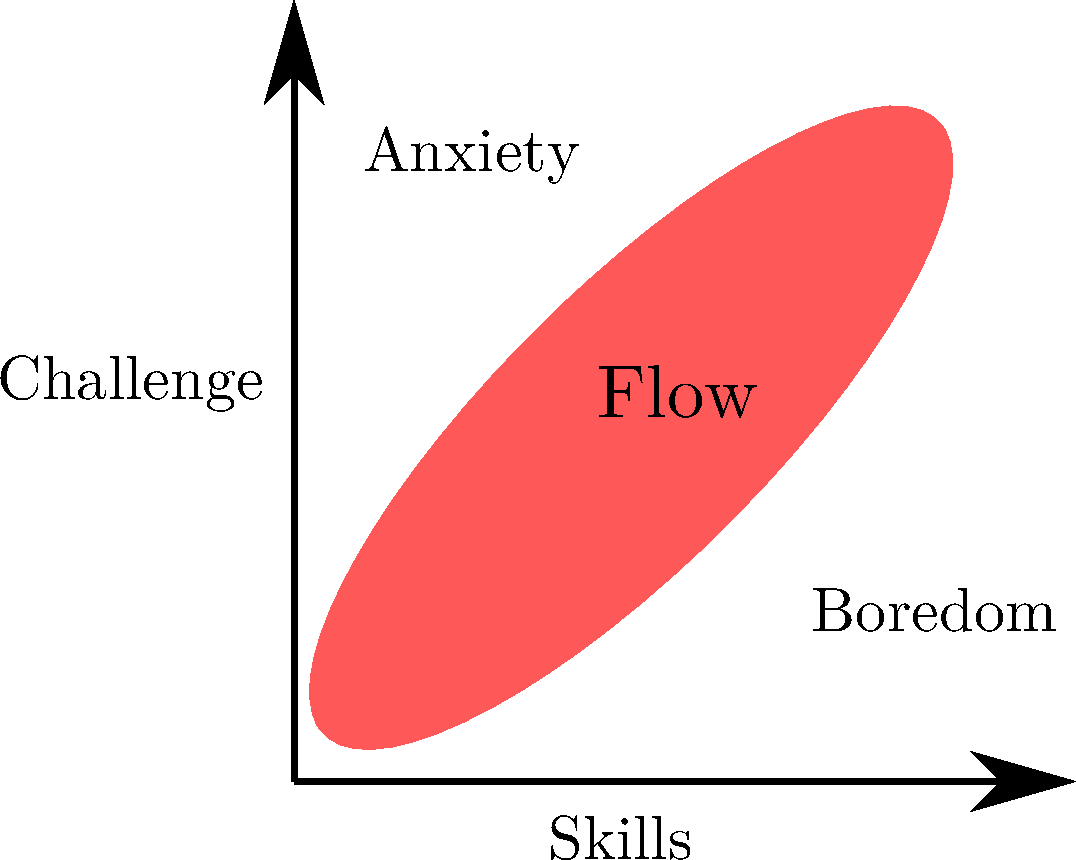
\includegraphics[width=\textwidth]{flow}
\label{fig:flow}
\caption[Short description found in the fig. table]{Long description, next to the figure}
\end{marginfigure}



\lipsum[1-3]

\begin{figure}[h!]
\begin{center}
\includegraphics[width=\textwidth]{NG2_alpha}
\end{center}
\caption[Short description found in the fig. table]{Long description, next to the figure}
\label{fig:NG_overview}
\end{figure}

\begin{figure*}[h!]
\begin{center}
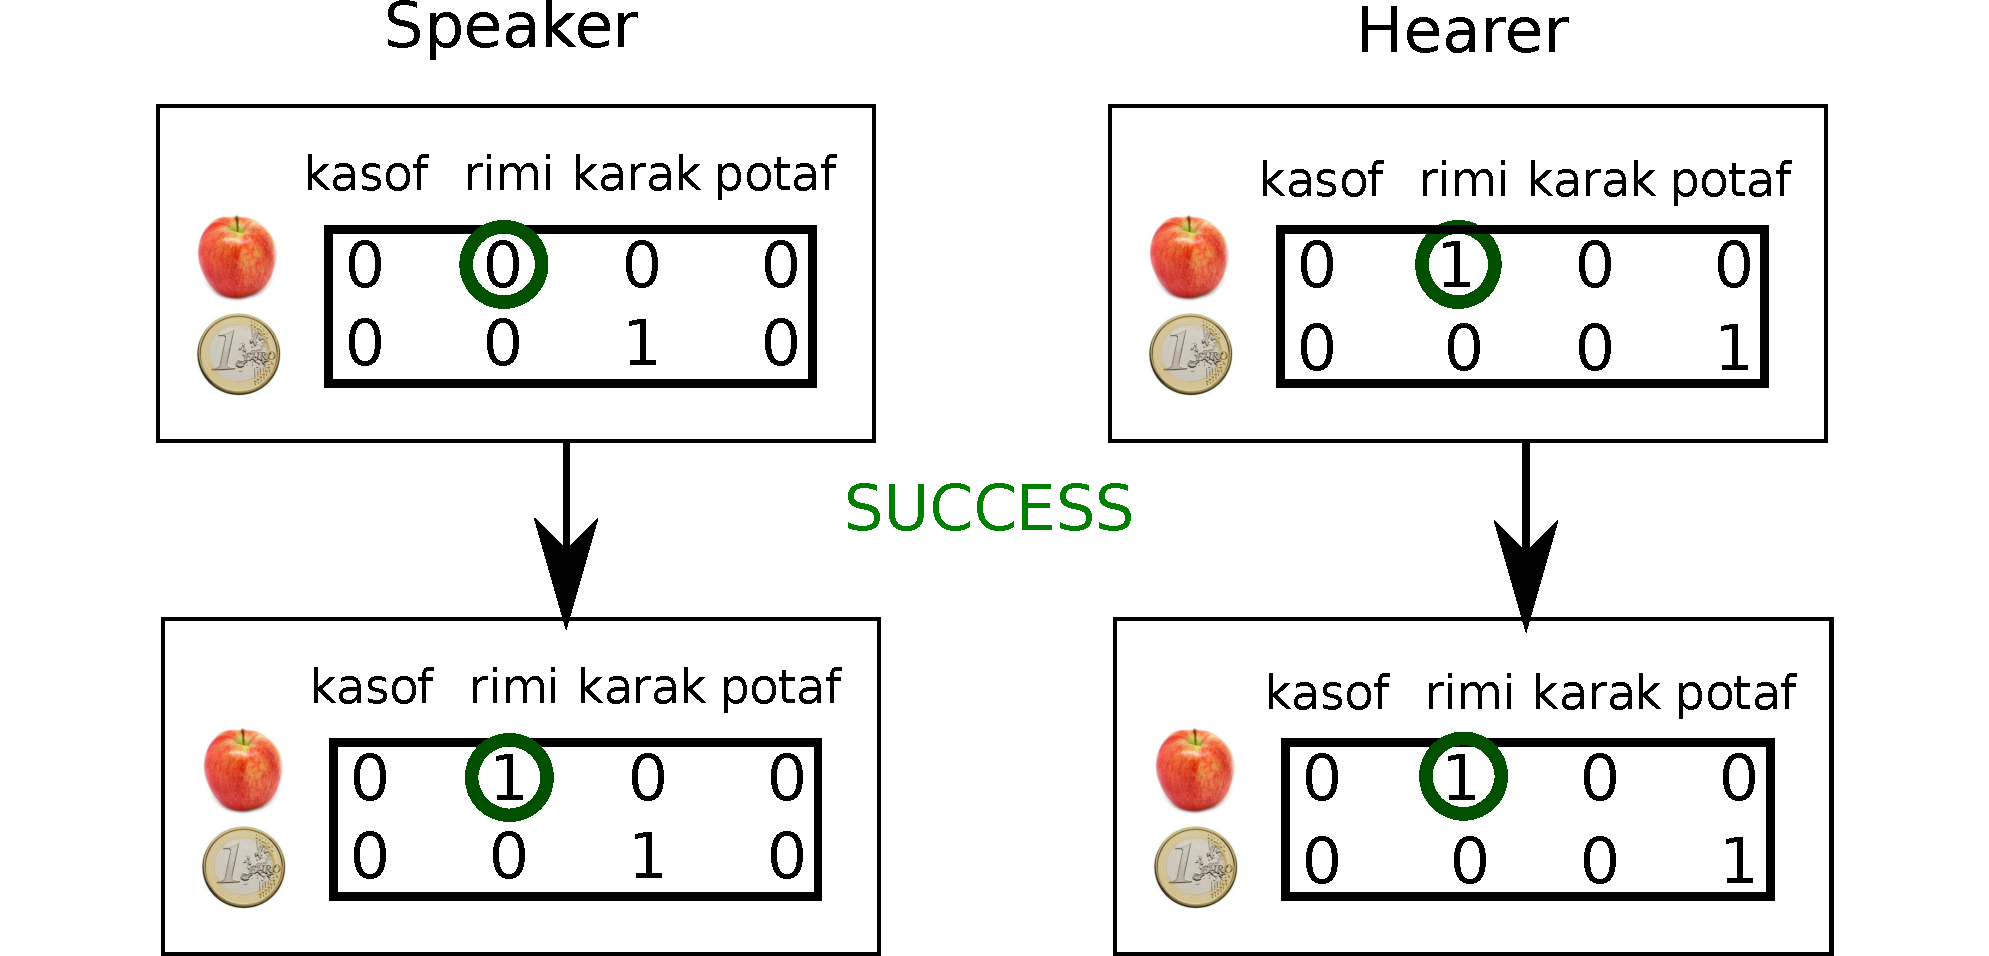
\includegraphics[width=0.5\textwidth]{success}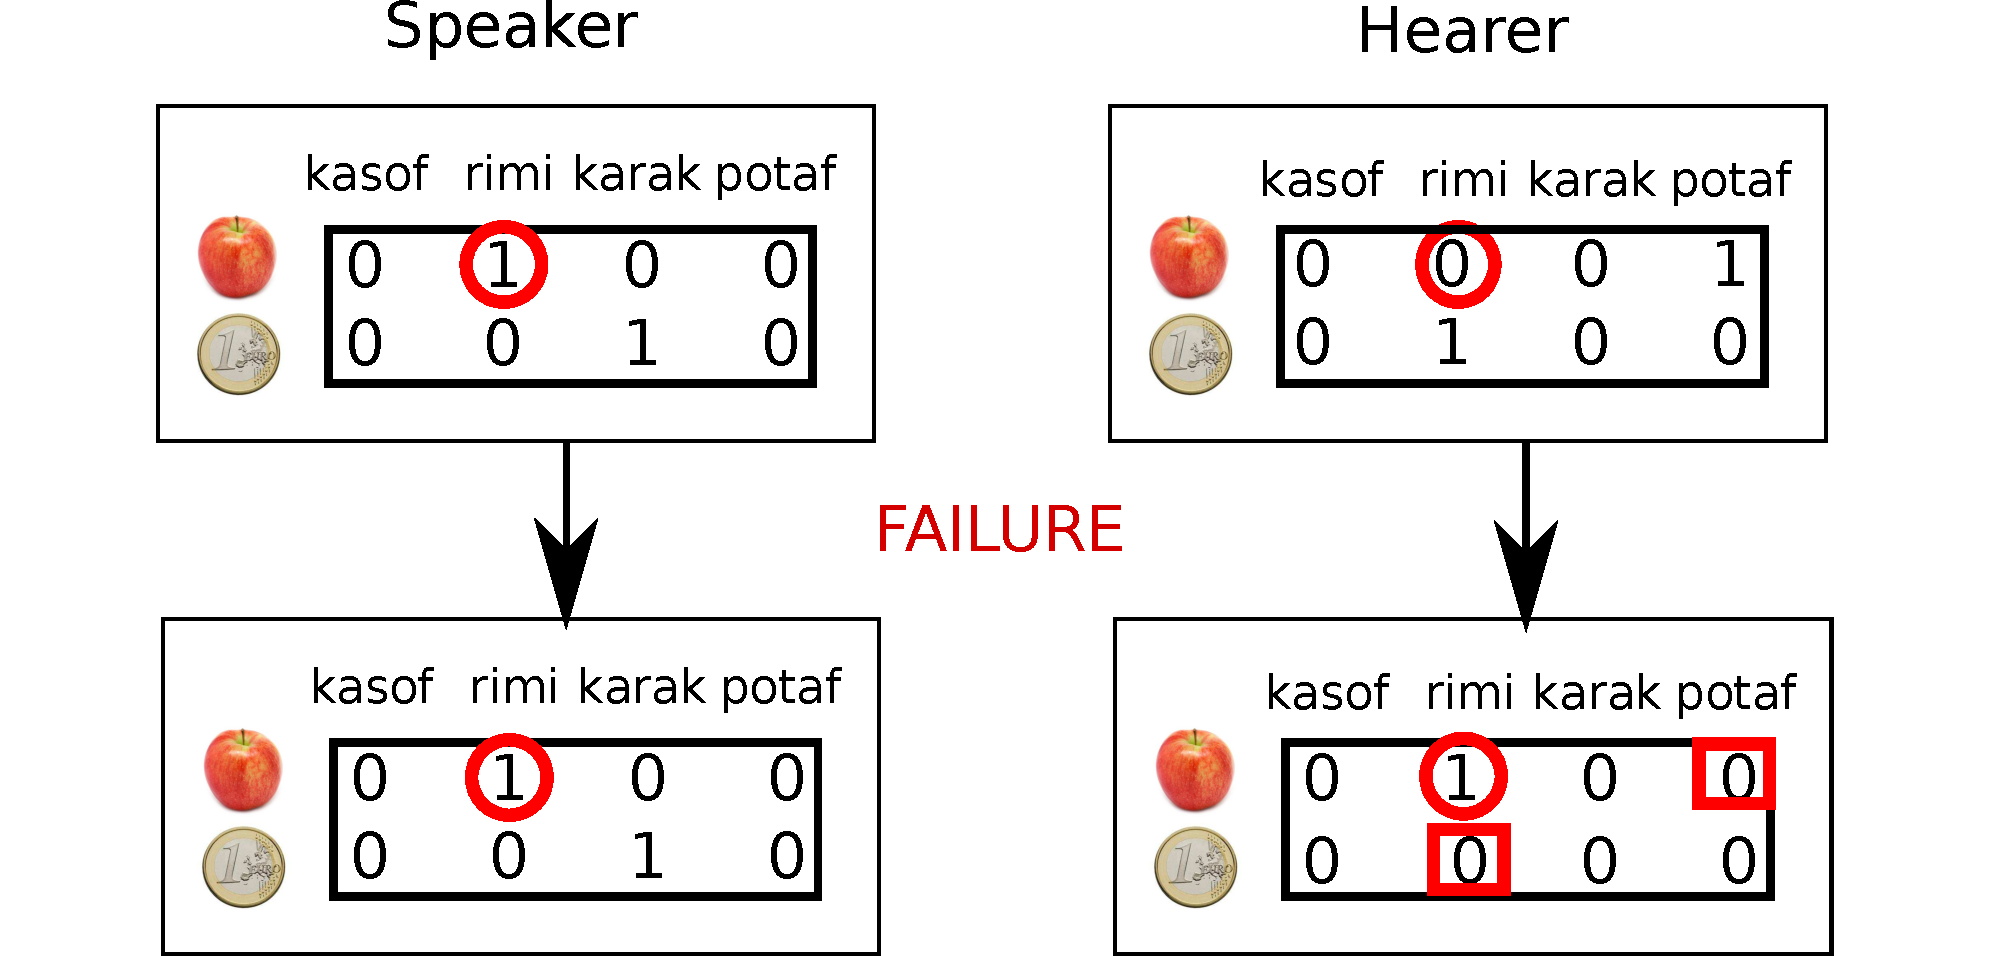
\includegraphics[width=0.5\textwidth]{fail}
\end{center}
\caption[Short description found in the fig. table]{Long description, next to the figure}
\label{fig:vocupdate}
\end{figure*}


\section{This thesis}

\subsection{Overview and structure}

This thesis introduces that, does this, and is awesome because blah. (Two general sentences to describe the work; then the content of each chapter can be described independently)

Chapter \ref{chap:chap1_fake} is a completely fake chapter with only a lorem ipsum.

Chapter \ref{chap:chap2_fake} is just the same.

\subsection{Contributions}

\begin{description}

\item[Contribution1:] \lipsum[1]

\item[Contribution2:] \lipsum[1]

\item[Contribution3:] \lipsum[1]


\end{description}

\subsection{Publications}

\begin{itemize}
\item \fullcite{schueller2015active}
\item \fullcite{schueller2016active}
\item \fullcite{schueller2018complexity}
\end{itemize}



\section{Short summary}

\lipsum[1-5]


\beforechapterpic{images/como.png}{Example illustration}
\part{A second part}

\beforechapterpic{images/bayou2.png}{Example illustration}

\chapter{First fake chapter\label{chap:chap1_fake}}
\minitoc

\section{First section}

\subsection{Subsection 1}

\lipsum[1-10]

\subsection{Subsection 2}

\lipsum[1-10]

\section{Second section}

\lipsum[1-10]


\beforechapterpic{images/kreyon.png}{Example illustration}

\chapter{Second fake chapter\label{chap:chap2_fake}}
\minitoc

\section{First section}

\subsection{Subsection 1}

\lipsum[1-10]

\subsection{Subsection 2}

\lipsum[1-10]

\section{Second section}

\lipsum[1-10]


\beforechapterpic{images/bcn.png}{Example illustration}
\part{Conclusions and Perspectives}
\beforechapterpic{images/cogsci.png}{Example illustration}

\chapter{Conclusion}
\minitoc

\lipsum[1-10]

\beforechapterpic{images/torun.png}{Example illustration}
\chapter{Future perspectives}


\lipsum[1-10]



\appendix

\beforechapterpic{images/koffel.png}{Example illustration}
\chapter{An open-source simulation framework \label{app:software}}
\minitoc

\section{First section}

\subsection{Subsection 1}

\lipsum[1-10]

\subsection{Subsection 2}

\lipsum[1-10]

\section{Second section}

\lipsum[1-10]

\backmatter
\setboolean{@mainmatter}{true}
\printbibliography

\setboolean{@mainmatter}{false}


\section*{Table of symbols}
\begin{table*}
\begin{tabular}{ll}

$\mathfrak{M}\;\;\;$ & Meaning space\\
$M\;\;\;$ & Size of the meaning space\\
$\mathfrak{M}_k\;\;\;$ & Set of known meanings\\
$\mu\;\;\;$ & Number of known meanings\\
$\mathfrak{M}_u\;\;\;$ & Set of unknown meanings\\
$m_i\;\;\;$ & Element of the meaning space\\
$\mathfrak{W}\;\;\;$ & Word space\\
$W\;\;\;$ & Size of the word space\\
$w_i\;\;\;$ & Element of the word space\\
$m_S\;\;\;$ & Meaning picked by the speaker, or topic\\
$m_H\;\;\;$ & Meaning interpreted by the hearer\\
$S\;\;\;$ & Speaker (one of the two possible roles in a Naming Game interaction)\\
$H\;\;\;$ & Hearer (one of the two possible roles in a Naming Game interaction)\\
$t$ & time, in total number of interactions\\
$S(t)\;\;\;$ & Theoretical Communicative Success measure\\
$t_{conv}\;\;\;$ & Time when reaching a global agreement: every agent has the same completed lexicon.\\
$S_{LAPS}(t)$ & Local Approximated Probability of Success measure\\
$S_{O}(t)$ & Observed Communicative Success\\
$N_l(t)\;\;\;$ & Local Complexity measure\\
$N_l^{max}\;\;\;$ & Maximum of Local Complexity measure\\
$t_{max}\;\;\;$ & Time when reaching the maximum of Local Complexity measure\\
$N_d(t)\;\;\;$ & Global Complexity measure\\
$N_d^{max}\;\;\;$ & Maximum of Global Complexity measure\\
$t_{GC}\;\;\;$ & Time when reaching the maximum of Local Complexity measure\\
$N_{inv}\;\;\;$ & Number of inventions during a Naming Game\\
$n_{ch}\;\;\;$ & Number of chunks for the Chunks strategy, depending on $N$ and $W$\\
$\alpha_{ST}\;\;\;$ & Parameter for the Success Threshold, normalized (divided by $N$)\\
$n_{MC}\;\;\;$ & Parameter for the minimal counts strategy\\
$\widetilde{n}_{MC}\;\;\;$ & Parameter for the Minimal Counts strategy, normalized (divided by $N$)\\
$\tau\;\;\;$ & Time scale parameter for LAPSmax and Coherence strategies\\


\end{tabular}
\caption[Table of symbols]{}
\label{tab:symbols}
\end{table*}

\clearpage
\section*{Table of Abbreviations and Acronyms}
\begin{table*}

\begin{tabular}{ll}

$MAB$ & Multi-Armed Bandit\\
$LAPS$ & Local Approximated Probability of Success\\
$ATC\;\;\;$  & Active Topic Choice\\
$RTC\;\;\;$  & Random Topic Choice\\
$AP\;\;\;$  & Acceptance Policy\\
$NG\;\;\;$ & Naming Game\\
$BLIS\;\;\;$ & Basic Lateral Inhibition Stategy, a vocabulary update policy\\
$TCS\;\;\;$ & Theoretical Communicative Success measure\\
$LC\;\;\;$ & Local Complexity measure\\
$GC\;\;\;$ & Global Complexity measure\\

\end{tabular}
\caption[Table of abbreviations and acronyms]{}
\label{tab:acronyms}
\end{table*}

% \printindex

\lastpic{images/istanbul.png}{A backcover illustration}
\setboolean{@mainmatter}{true}
\end{document}
